\begin{news}
{2} %columnes
{Crònica de la Torronada 2010}
%index: Torranda
{ \noindent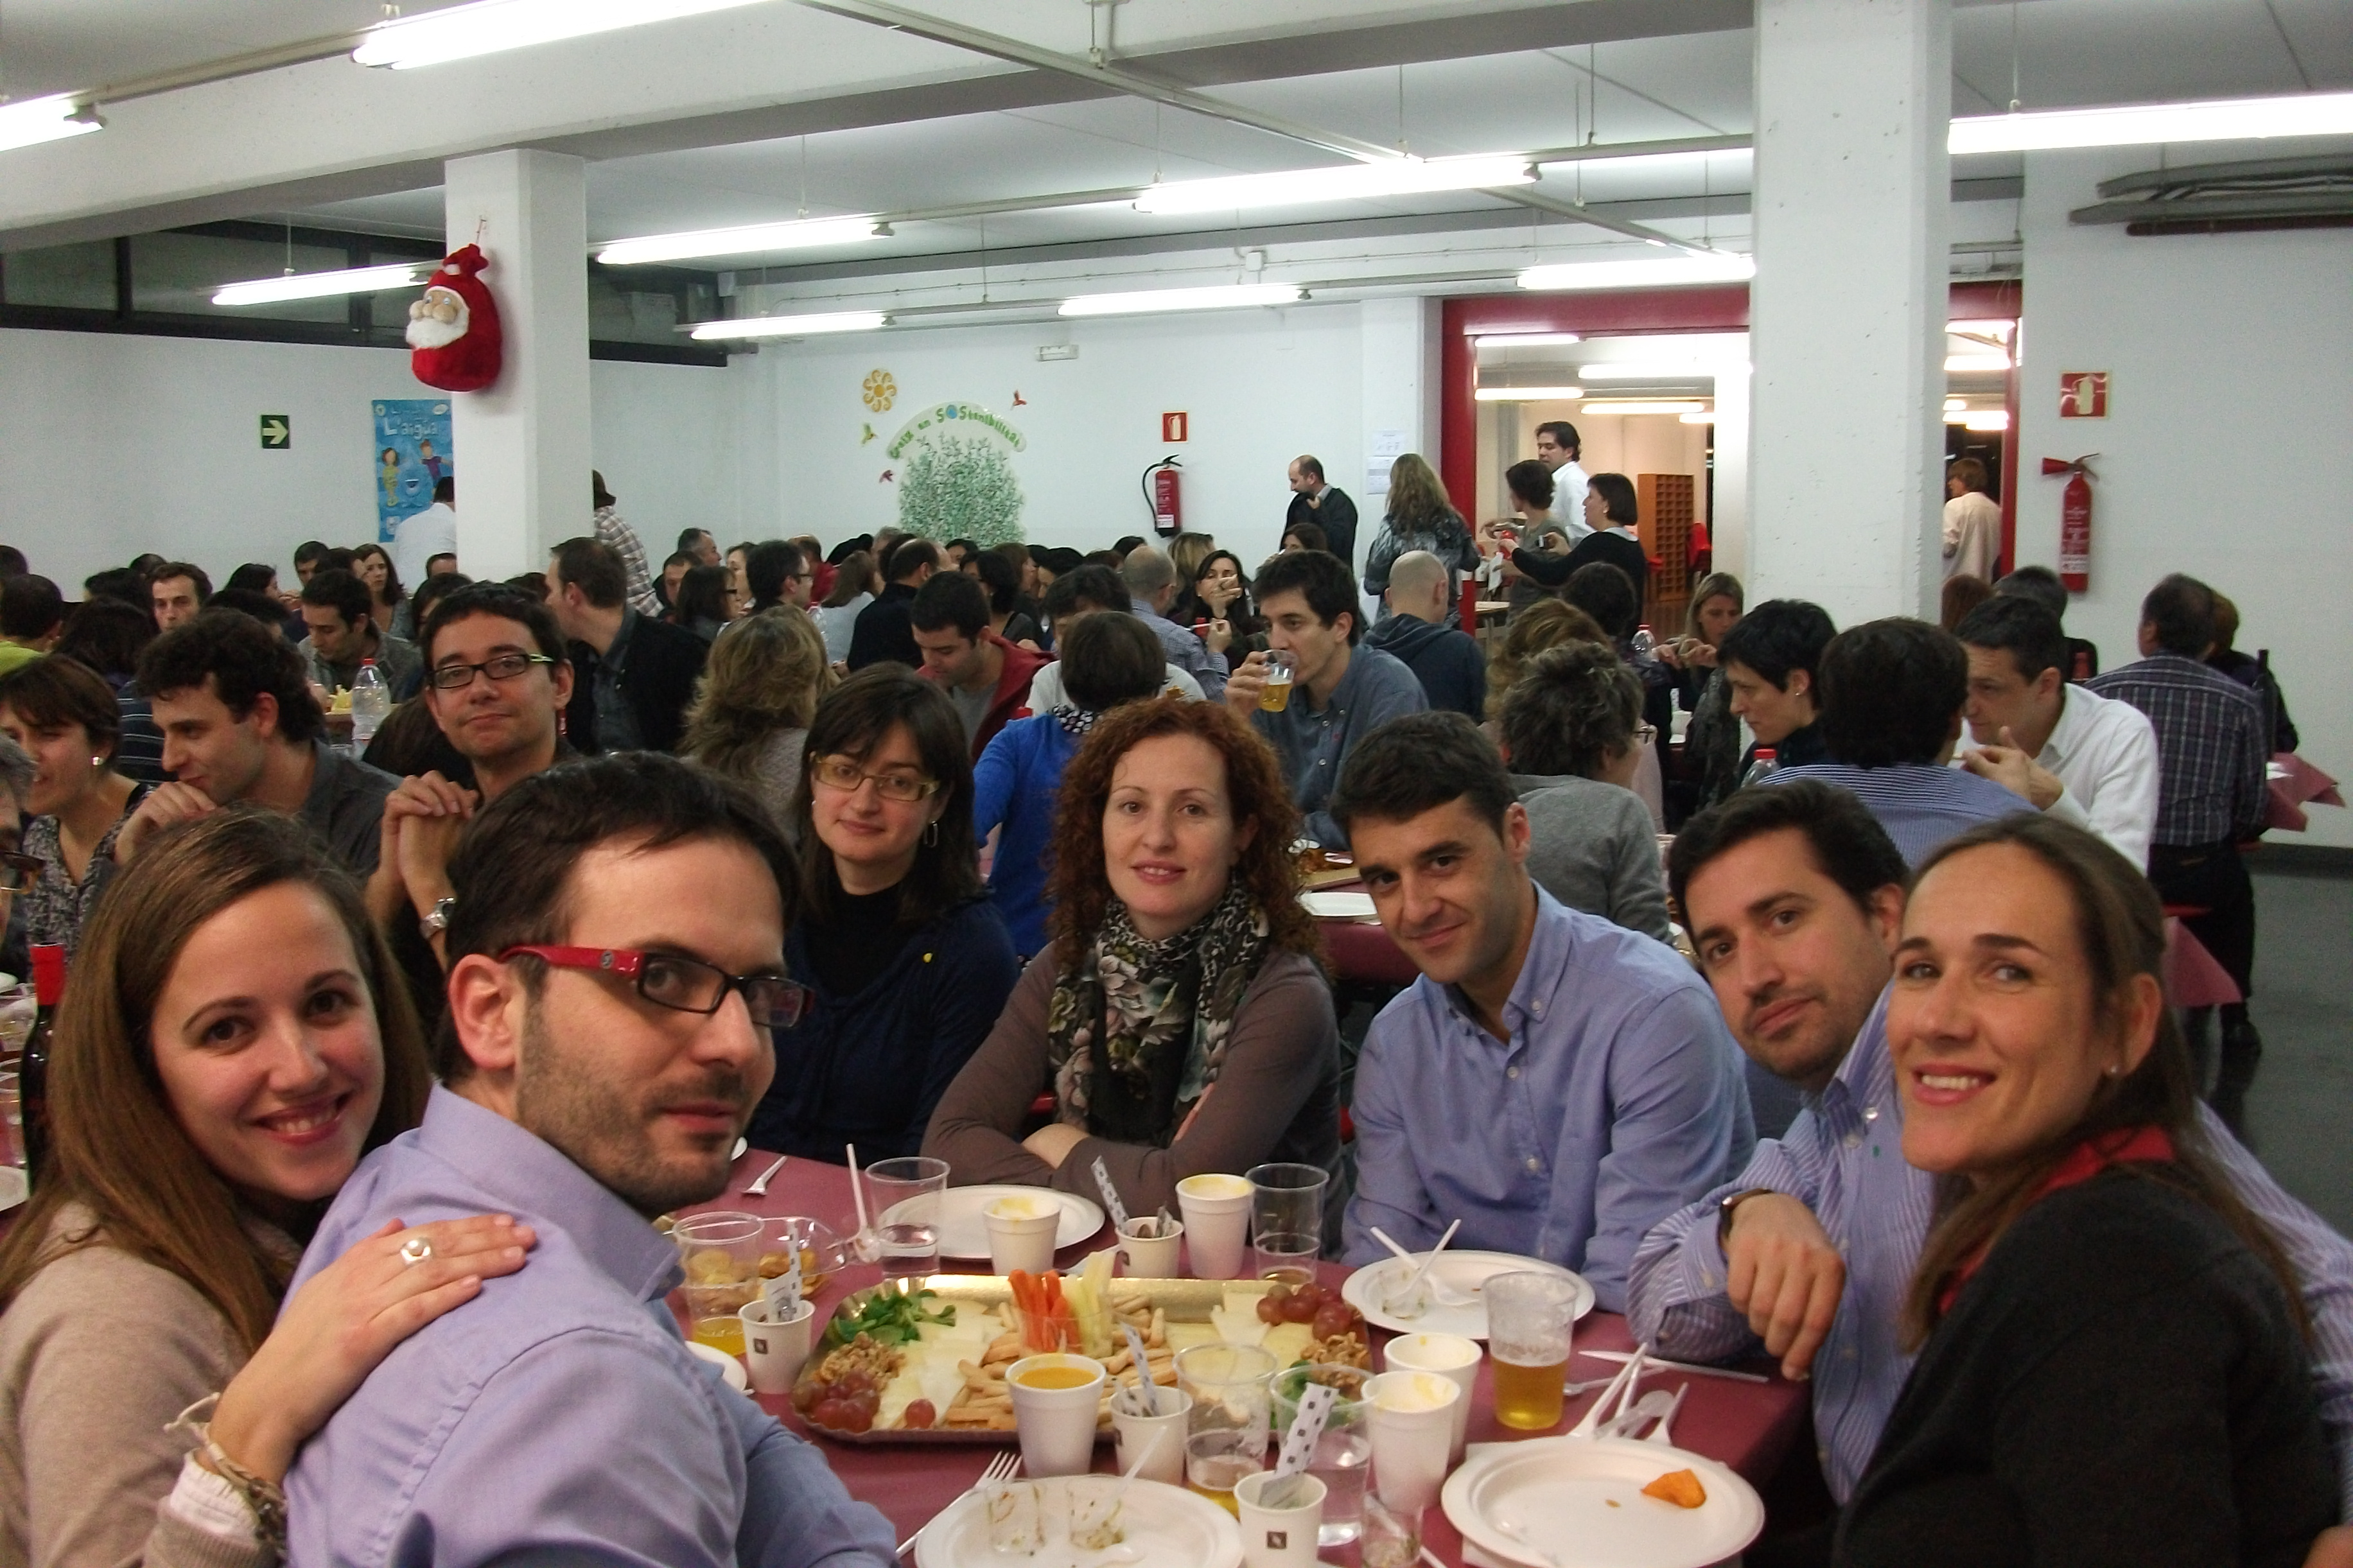
\includegraphics[width=18.2cm,keepaspectratio]{ampa/img/DSCF0909.JPG}}
{Fem Escola}
{609} %pagesof

Un èxit sense precedents! Per fi la Torronada aconsegueix reunir més de 125 mares, pares i mestres de l’escola!

El menjador es va  vestir de gala: estovalles vermelles, safates plenes de viandes, pares i mares amunt i avall, organitzant les taules, servint el sopar, preparant el cafès i… tallant torrons ( en honor al nom de la festa) , no hi podien faltar.

Aquest any sabíem que la torronada seria diferent…, coses per celebrar i molta gent animada s’havia apuntat, això sÍ , tothom amb la pandereta, què ens estarà esperant? 

El sopar, un encert, i després toca formar els grups. 6 colors, 6 nadales, 10 minuts per assajar, la glòria ens està esperant…Fem la ronda, i ja tenim un guanyador, el grup vermell amb una actuació magistral de “Los peces en el rio” s’alça amb el premi, un magnífic Panettone, que vam gaudir  tots plegats.

I després del sopar, la tertúlia i el concurs, comença la marxa, fins que aguanti el cos.

Cal que els anys no ens treguin la il·lusió…això només és el principi!!!

\columntitle{lines}{
Gràcies a tots els que ho heu fet possible! 
MOLT BON NADAL I EL MILLOR PER A L’ANY NOU!
}

\authorandplace{Text: Gemma López - Fotos: Silvia Serra}{Mares de P5}

\noindent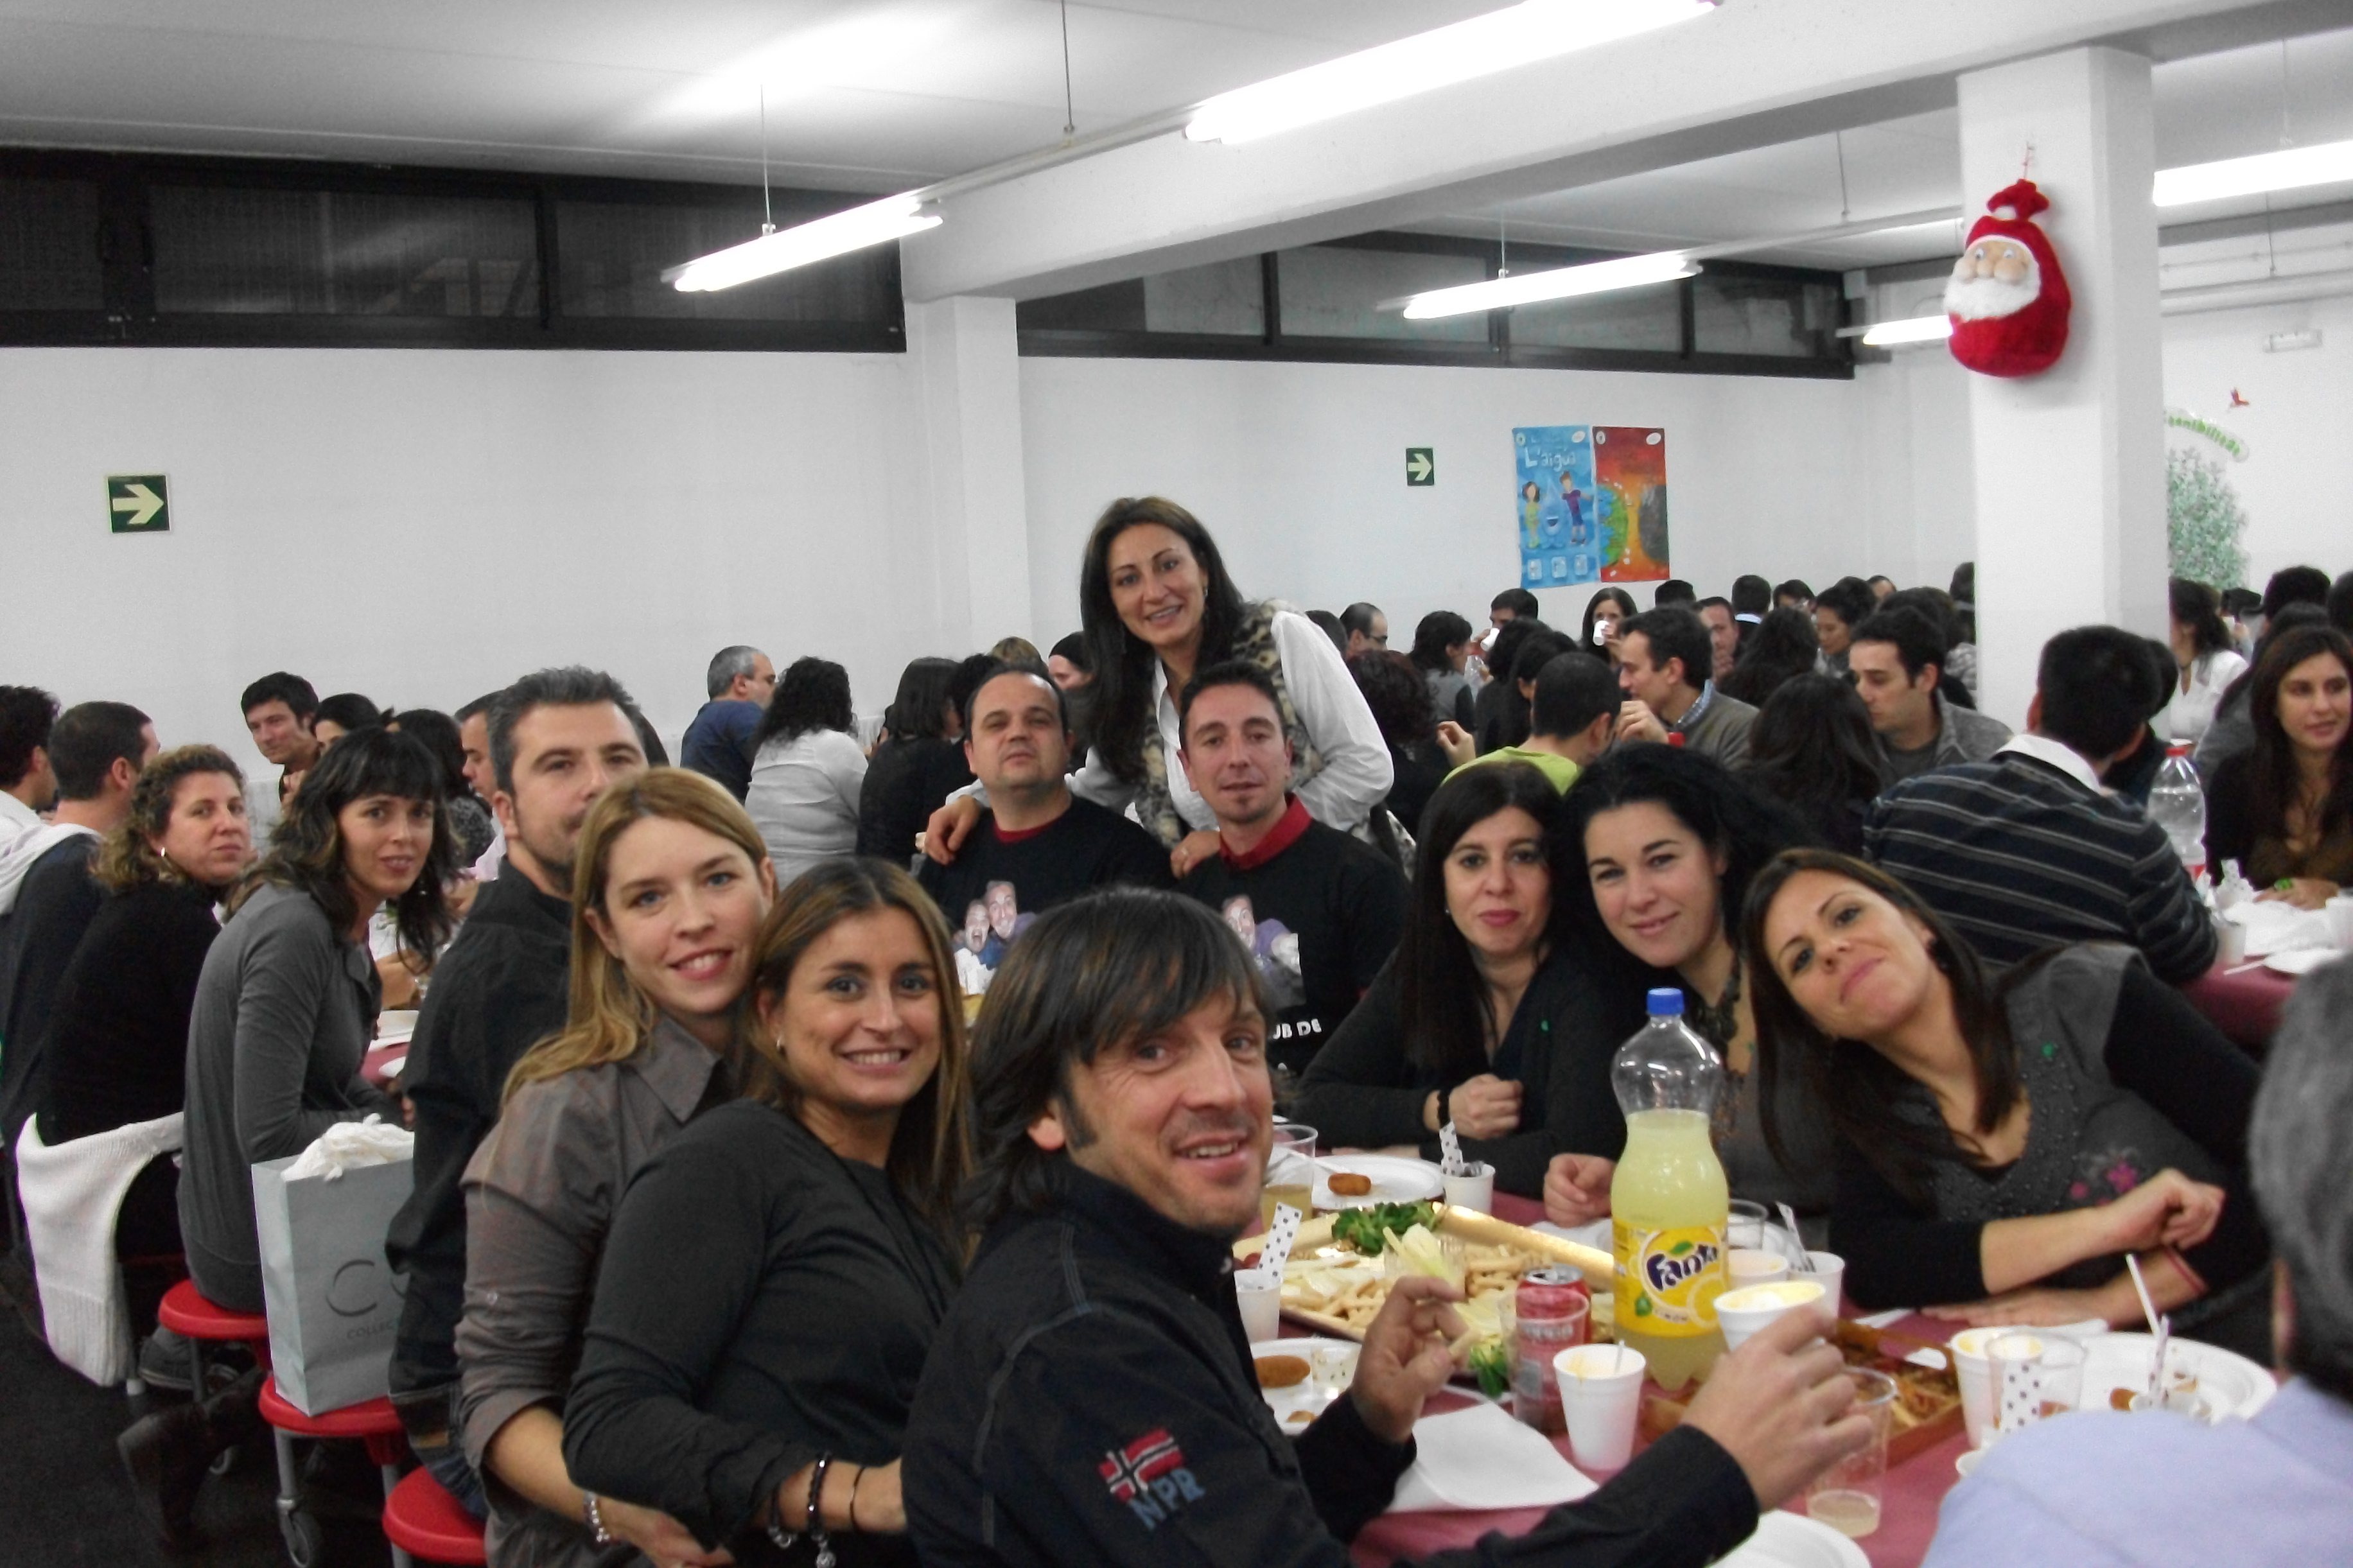
\includegraphics[width=9cm,keepaspectratio]{ampa/img/DSCF0911.JPG}

\noindent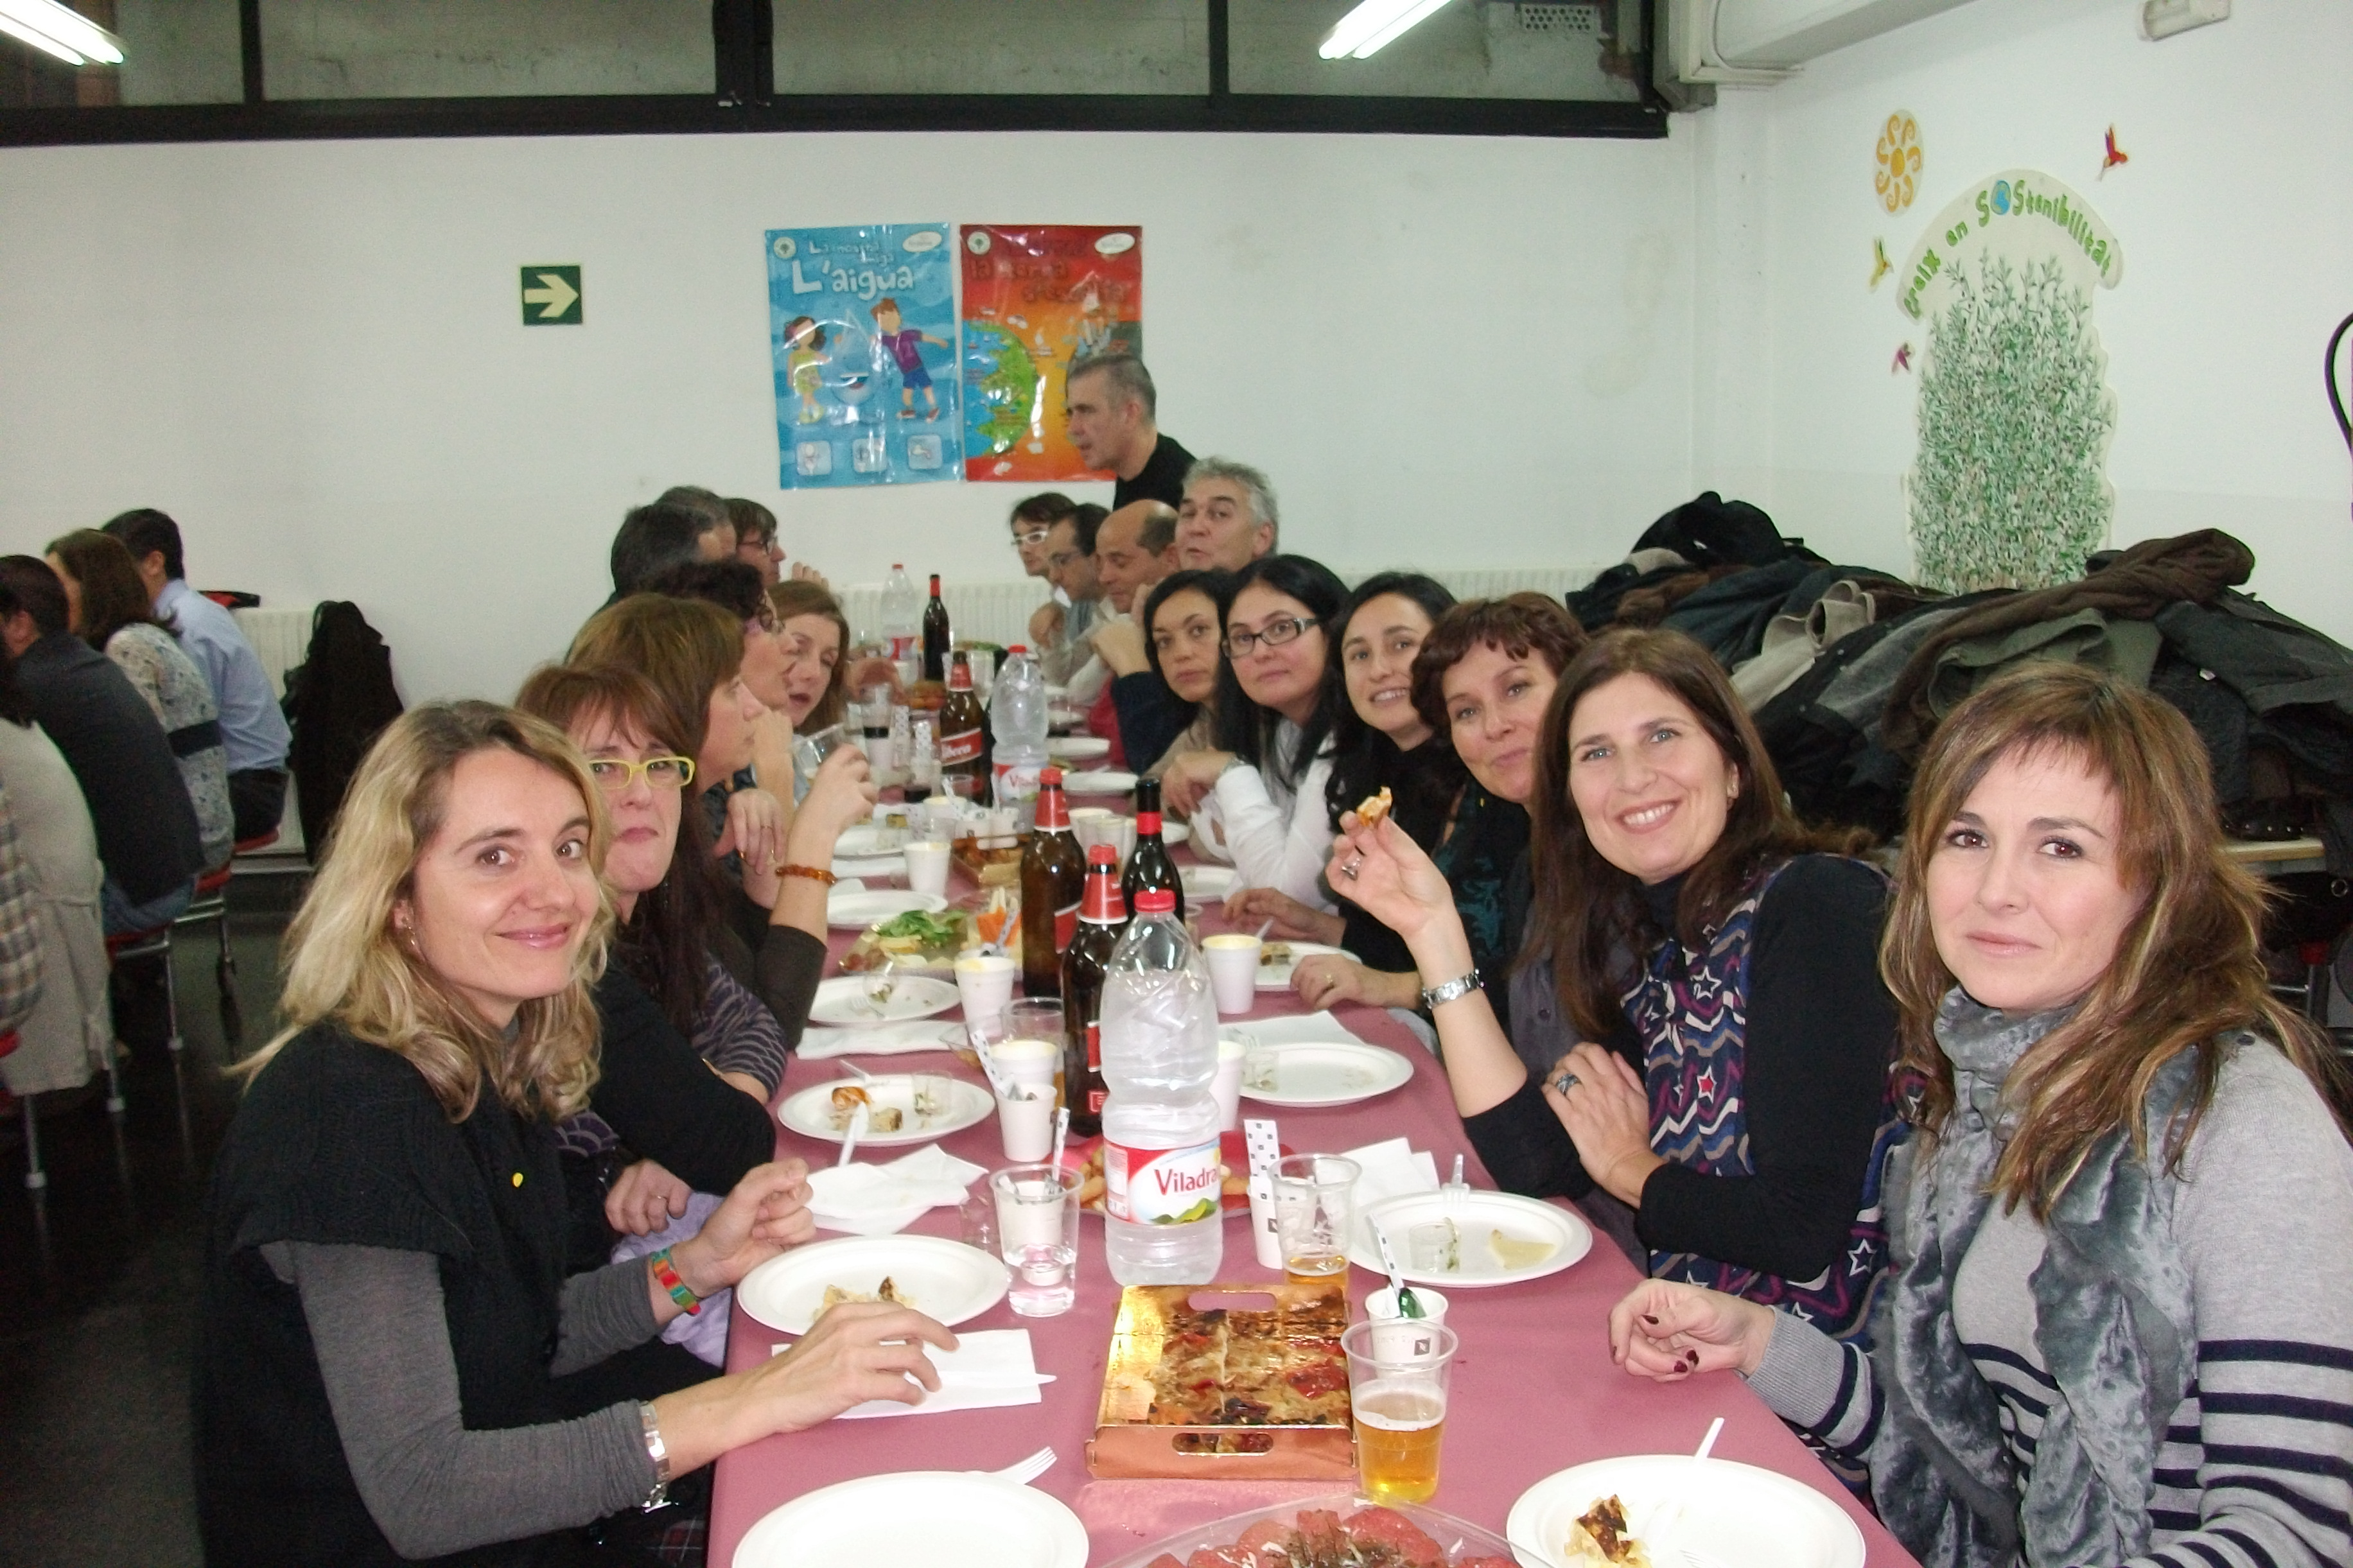
\includegraphics[width=9cm,keepaspectratio]{ampa/img/DSCF0920.JPG}


\end{news}
